\documentclass{SciPost}

% Prevent all line breaks in inline equations.
%\binoppenalty=10000
%\relpenalty=10000

\hypersetup{
    colorlinks,
    linkcolor={red!50!black},
    citecolor={blue!50!black},
    urlcolor={blue!80!black}
}

\usepackage[bitstream-charter]{mathdesign}
\urlstyle{same}

% Fix \cal and \mathcal characters look (so it's not the same as \mathscr)
\DeclareSymbolFont{usualmathcal}{OMS}{cmsy}{m}{n}
\DeclareSymbolFontAlphabet{\mathcal}{usualmathcal}

\fancypagestyle{SPstyle}{
\fancyhf{}
\lhead{\colorbox{scipostblue}{\bf \color{white} ~Notes on Physics}}
\rhead{{\bf \color{scipostdeepblue} ~Nonequilibrium}}
\renewcommand{\headrulewidth}{1pt}
\fancyfoot[C]{\textbf{\thepage}}
}

\begin{document}

\pagestyle{SPstyle}

\begin{center}{\Large \textbf{\color{scipostdeepblue}{
Information Scrambling in Chaotic Systems\\
}}}\end{center}

\begin{center}
\textbf{Jie Ren}
\end{center}

\tableofcontents

\section{Weingarten Calculus}

This section discusses the techniques for averaging random unitary operators appearing in various chaotic models.
\begin{equation}
	\left\langle U_{i_1 j_1} \cdots U_{i_n j_n} U_{i_1^{\prime} j_1^{\prime}}^* \cdots U_{i_n^{\prime} j_n^{\prime}}^* \right\rangle_\text{Haar}
	\equiv \int_{U_d} dU \ U_{i_1 j_1} \cdots U_{i_n j_n} U_{i_1^{\prime} j_1^{\prime}}^* \cdots U_{i_n^{\prime} j_n^{\prime}}^*
\end{equation}
We will review a standard formula for the average of matrix elements of the unitary matrix concerning the Haar probability measure.

The central quantity we need is the \textbf{Weingarten functions}, which appear when we are evaluating the following integrals:
\begin{equation}\label{eq:haar-integral}
	\left\langle U_{i_1 j_1} \cdots U_{i_n j_n} U_{i_1^{\prime} j_1^{\prime}}^* \cdots U_{i_n^{\prime} j_n^{\prime}}^* \right\rangle_\text{Haar}
	= \sum_{\sigma, \tau \in S_k} \delta_{i_1 i_{\sigma(1)}^{\prime}} \cdots \delta_{i_n i_{\sigma(n)}^{\prime}} \delta_{j_1 j_{\tau(1)}^{\prime}} \cdots \delta_{j_n j_{\tau(n)}^{\prime}} \operatorname{Wg}_d\left(\sigma \tau^{-1}\right),
\end{equation}
where $\operatorname{Wg}_d(g)$ is the Weingarten function.
In practice, we usually encounter cases where $q\le 2$.
For the ($n=1$) case, the only Weingarten function is
\begin{equation}
	\operatorname{Wg}_d([1]) = \frac{1}{d} \quad\Longrightarrow\quad
	\langle U_{i j} U_{i^{\prime} j^{\prime}}^* \rangle = \frac{1}{d}\delta_{ii'}\delta_{jj'}.
\end{equation}
For the ($n=2$) case, the Weingarten functions are
\begin{equation}
	\operatorname{Wg}_d([2])=\frac{-1}{d\left(d^2-1\right)}, \quad
	\operatorname{Wg}_d\left([1,1]\right)=\frac{1}{d^2-1},
\end{equation}
which leads to the following Haar measure integral:
\begin{equation}
\begin{aligned}
	\left\langle U_{i_1 j_1} U_{i_2 j_2} U_{i_1^{\prime} j_1^{\prime}}^* U_{i_2^{\prime} j_2^{\prime}}^* \right\rangle_\text{Haar}
	=&\ \frac{
		\delta_{i_1 i'_1}\delta_{i_2 i'_2}\delta_{j_1 j'_1}\delta_{j_2 j'_2} + 
		\delta_{i_1 i'_2}\delta_{i_2 i'_1}\delta_{j_1 j'_2}\delta_{j_2 j'_1}
	}{d^2-1} \\
	& -\frac{
		\delta_{i_1 i'_2}\delta_{i_2 i'_1}\delta_{j_1 j'_1}\delta_{j_2 j'_2} + 
		\delta_{i_1 i'_1}\delta_{i_2 i'_2}\delta_{j_1 j'_2}\delta_{j_2 j'_1}
	}{d(d^2-1)}.
\end{aligned}
\end{equation} 

\subsection{Explicit form}
Formally, $\operatorname{Wg}_d(g)$ has the closed form
\begin{equation}
	\operatorname{Wg}_d(g)=\frac{1}{n!} \sum_{\lambda} \frac{\chi_\lambda(e) \chi_\lambda(g)}{\prod_{(i, j) \in Y(\lambda)}(d-i+j)},
\end{equation}
where 
\begin{itemize}
	\item the sum is over all partitions $\lambda=[\lambda_1,\cdots,\lambda_l]$ of $n=\sum_i\lambda_i$;
	\item a partition $\lambda$ specifies a Young diagram $Y(\lambda)$, and also corresponds to an irreducible representation.
	\item $\chi_\lambda(g)$ is the irreducible character of the symmetric group $S_n$ indexed by the partition $\lambda$;
	\item $(i,j)\in Y(\lambda)$ stands for $1\le i\le l$, $1\le j\le \lambda_i$, i.e., the coordinate of the Young diagram.
\end{itemize}
Note that $\operatorname{Wg}_d(g)$ is related only to the character, so it is a function of classes.

Let us give a few examples. 
For ($n=1$), the partition can only be $\lambda=[1]$, which is a trivial representation:
\begin{equation}
	\chi_{[1]}(e)=1 \quad\Longrightarrow\quad \mathrm{Wg}_d([1])=\frac{1}{d}.
\end{equation}

For ($n=2$), the partition can be $\lambda=[2]$ or $\lambda=[1,1]$, corresponding to the character table:
\begin{equation*}
\begin{tabular}{M{3cm}|M{2cm}M{2cm}c}
	\hline\hline
	Representation & $e$ & $\sigma$ & \\
	\hline \\ [-10pt]
	$[2]$ & $1$ & $1$ & \\[3pt]
	$[1,1]$ & $1$ & $-1$ & \\[3pt]
	\hline\hline
\end{tabular}
\end{equation*}
Therefore, the explicit calculation leads to
\begin{equation*}
\begin{aligned}
	\operatorname{Wg}_d(e) &=\frac{1}{2} \left[\frac{1}{d(d+1)}+\frac{1}{d(d-1)}\right]= \frac{1}{d^2-1}, \\
	\operatorname{Wg}_d(\sigma) &=\frac{1}{2} \left[\frac{1}{d(d+1)}-\frac{1}{d(d-1)}\right]= \frac{-1}{d(d^2-1)}.
\end{aligned}
\end{equation*}

For ($n=3$), the character table for $S_3$ is
\begin{equation*}
\begin{tabular}{M{3cm}|M{2cm}M{2cm}M{2cm}c}
	\hline\hline \\ [-10pt]
	Representation & $e$ & $(1,2)$ & $(1,2,3)$ & \\ [1pt]
	\hline \\ [-10pt]
	$[2]$ & $1$ & $1$ & $1$ & \\[3pt]
	$[1^3]$ & $1$ & $-1$ & $1$ & \\[3pt]
	$[2,1]$ & $2$ & $0$ & $0$ & \\[3pt]
	\hline\hline
\end{tabular}
\end{equation*}
The direct calculation then gives
\begin{equation*}
\begin{aligned}
	\operatorname{Wg}_d(e) 
	&=\frac{1}{6} \left[\frac{1}{d(d+1)(d+2)}+\frac{1}{d(d-1)(d-2)}+\frac{4}{d(d+1)(d-1)}\right]
	= \frac{d^2-2}{d(d^2-1)(d^2-4)}, \\
	\operatorname{Wg}_d((12)) 
	&=\frac{1}{6} \left[\frac{1}{d(d+1)(d+2)}-\frac{1}{d(d-1)(d-2)}\right]
	= \frac{-1}{(d^2-1)(d^2-4)}, \\
	\operatorname{Wg}_d((123)) 
	&=\frac{1}{6} \left[\frac{1}{d(d+1)(d+2)}+\frac{1}{d(d-1)(d-2)}-\frac{2}{d(d+1)(d-1)}\right]
	= \frac{2}{d(d^2-1)(d^2-4)}.
	\end{aligned}
\end{equation*}
One useful property of the Weingarten function is the 
\begin{equation}
	\operatorname{Wg}_d(g) = d^{-n-|g|} \prod_i (-1)^{|C_i|-1}c_{|C_i|-1} + O(d^{-n-|d|-2}),
\end{equation}
where $g$ is a product of cycles of length $C_i$, and $c_n = (2n)!/n!(n+1)!$ is the Catalan number, and $|g|$ is the smallest number of transpositions that $g$ is a product of.


\subsection{Orthogonal groups}
For integral over $O(d)$, 
\begin{equation}
	\mathbb E\left[O_{i_1j_1}\cdots O_{i_{2n}j_{2n}}\right]
	=\sum_{\sigma,\tau\in M_{2n}}
	\delta_{i_{\sigma(1)}i_{\sigma(2)}}\cdots\delta_{i_{\sigma(2n-1)}i_{\sigma(2n)}}
	\delta_{j_{\tau(1)}j_{\tau(2)}}\cdots\delta_{j_{\tau(2n-1)}j_{\tau(2n)}}
	\operatorname{Wg}_d^{O}(\sigma^{-1}\tau),
\end{equation}
where $M_{2n}$ is $S_{2n}$ mod all the switching of $(2n-1,2n)$ pairs, and $\operatorname{Wg}_d^{O}$ is the Weingarten function for orthogonal groups:
\begin{equation}
	\operatorname{Wg}_d^O(g) = \frac{1}{(2n)!}\sum_\lambda \frac{\chi_{2\lambda}(e) \sum_{\xi\in H_{n}} \chi_{\lambda}(g\xi)}{\prod_{(i,j)\in Y(2\lambda)}(d+2j-i-1)},
\end{equation}
where $H_n$ is generated by $\{(2i-2,2i),(2i-1,2j-1)(2i,2j)|i,j\le n\}$.

For ($n=1$) case, the Weingarten function is
\begin{equation}
	\operatorname{Wg}^O_d(e) = \frac{1}{d} \quad\Longrightarrow\quad
	\mathbb E\left[O_{i_1j_1}O_{i_2j_2}\right]
	= \frac{1}{d}\delta_{i_1i_2}\delta_{j_1j_2}.
\end{equation}

For ($n=2$) case, the partition $\lambda=[2]/[1,1]$, and $2\lambda=[4]/[2,2]$. 
\begin{equation}
	H_n=\{e,(12),(34),(12)(34),(13)(24),(14)(23),(1324),(1423)\}
\end{equation}
The characters we need are listed below:
\begin{equation*}
\begin{tabular}{M{2.6cm}|M{1cm}M{1cm}M{1.5cm}M{2cm}M{1.2cm}c}
	\hline\hline \\ [-10pt]
	Representation & $e$ & $(1,2)$ & $(1,2,3)$ & $(1,2)(3,4)$ & $(1,2,3,4)$ & \\ [1pt]
	\hline \\ [-10pt]
	$[4]$ & $1$ & $1$ & $1$ & $1$ & $1$ & \\[3pt]
	$[2^2]$ & $2$ & $0$ & $-1$ & $2$ & $0$ & \\[3pt]
	\hline\hline
\end{tabular}
\end{equation*}
Then, for the element $e$:
\begin{equation}
	\operatorname{Wg}^O_d(e) = \frac{1}{24}\left[\frac{8}{d(d+2)}+\frac{16}{d(d-1)}\right]
= \frac{d+1}{d(d+2)(d-1)}.
\end{equation}
Note that $\operatorname{Wg}^O_d$ is still a function of classes, and is also equal in the same coset $S_{2n}/H_n$.
\begin{equation}
	\operatorname{Wg}_d^{O}((23))= \frac{1}{24}\left[\frac{8}{d(d+2)}+\frac{-8}{d(d-1)}\right]
	= \frac{-1}{d(d+2)(d-1)}.
\end{equation}








\section{Applications for scrambled systems}







\subsection{Information scrambling by random unitaries}

Consider a mixed initial state (we consider an enlarged system as a purification of the mixed state, where the memory is an $s$-qubit system):
\begin{equation}
	|\Psi\rangle 
	= \frac{1}{\sqrt{2}}\left(|0\rangle_R U_{A} \otimes I_{\mathrm{MEM}}|0, \sqrt{\rho}\rangle+|1\rangle_R U_{A} \otimes I_{\mathrm{MEM}}|1, \sqrt{\rho}\rangle\right) 
	= 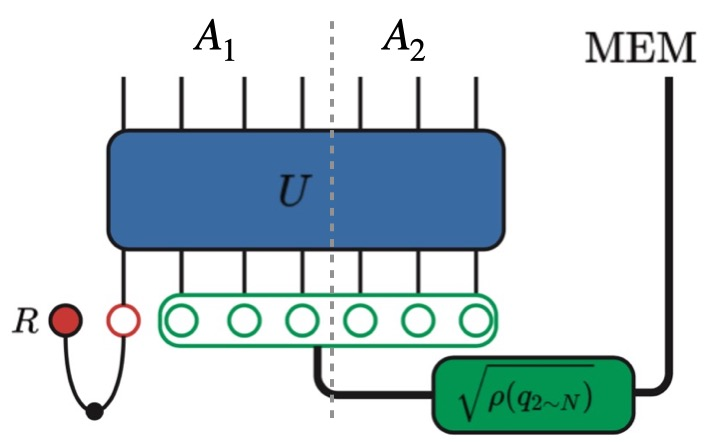
\includegraphics[align=c,width=0.25\linewidth]{pics/mixed-state.jpg},
\end{equation}
which contains a reference qubit $R$ maximally entangled with the first qubit of the system $A$.
Applying a random unitary evolution to system $A$, we ask how much information is shared between $R$ and part of the system $A_1$.

We can regard the subsystems $A_1$ and $A_2$ as two large indices.
When calculating $S^{(2)}_{A_1}$, we consider inner-product of the randomized state with boundary $\langle \mathbb I_R(12)_{A_1}\mathbb I_{A_2\cup\text{MEM}}|$.
Using the Weingarten calculus,
\begin{equation}\label{eq:alter-boundary}
	\sum_{\sigma, \tau \in S_2} \mathrm{Wg}_2\left(\tau \sigma^{-1}\right)
	\langle \mathbb (12)_{A_1} \mathbb I_{A_2}|\tau_{A} \rangle\langle\sigma_{A} |
	= \frac{|A|}{|A|^2-1} \left[\left(|A_1|-\frac{1}{|A_1|}\right) \langle(12)_A|+
	\left(|A_2|-\frac{1}{|A_2|}\right) \langle\mathbb I_A| \right],
\end{equation}
the averaging of the unitary gate effectively alters the boundary to the sum of $\langle \mathbb I_R(12)_{A}\mathbb I_\text{MEM}|$ and $\langle \mathbb I_{A\cup R\cup \text{MEM}}|$.
The averaged entropy of $A_1$ is then\footnote{Note that what we averaged is $\langle \rho^2_{A_1}\rangle$. We define a purity entropy $\tilde S^{(2)}_{A_1} \equiv -\log_2 \langle \rho^2_{A_1}\rangle$. While it is a good approximation of $S^{(2)}_{A_1}$ when the fluctuation is small.}
\begin{equation}
	2^{-\tilde S^{(2)}_{A_1}} 
	= \frac{|A|}{|A|^2-1}\left[\left(|A_1|-\frac{1}{|A_1|}\right)\tr\rho^2_A + \left(|A_2|-\frac{1}{|A_2|}\right)(\tr\rho)^2\right].
\end{equation}
Similarly, when considering the averaged purity entropy of subsystem $A_1 \cup R$, Eq.~(\ref{eq:random-unitary-gate}) changes the boundary from $\langle(12)_{R}\mathbb I_{A_1} (12)_{A_2}\mathbb I_\text{MEM}|$ to $\langle (12)_{A\cup R}\mathbb I_\text{MEM}|$ and $\langle(12)_{R}\mathbb I_{A\cup \text{MEM}}|$, i.e.,
\begin{equation}
\begin{aligned}
	2^{-\tilde S^{(2)}_{A_1\cup R}} 
	= \frac{|A|}{|A|^2-1}\left[\left(|A_1|-\frac{1}{|A_1|}\right)\tr\rho^2_{A\cup R}+\left(|A_2|-\frac{1}{|A_2|}\right)\tr\rho^2_R\right].
\end{aligned}
\end{equation}
We can quantify the information scrambling by calculating the averaged (purity) mutual information
\begin{equation}
\begin{aligned}
	\tilde I^{(2)}(A_1: R) &\equiv \tilde S^{(2)}_{A_1} + \tilde S^{(2)}_{R} - \tilde S^{(2)}_{A_1\cup R}
	= \tilde S^{(2)}_{A_1} - \tilde S^{(2)}_{A_1\cup R} + 1 \\
	&= 1 + \log_2 \left[2-\frac{3}{2}\frac{(2^{\alpha N}-2^{-\alpha N})}{(2^{\alpha N}-2^{-\alpha N})+[2^{(1-\alpha)N} - 2^{-(1-\alpha)N}]2^{-s-1}}\right].
\end{aligned}
\end{equation}
where we assuming $A$ has $N$ qubits and $A_2$ has $\alpha N$ qubits.

A few remarks are in order.
First, when we consider the pure initial state ($s=0$), the expression is reduced to
\begin{equation}
	\tilde I^{(2)}(A_1: R)
	= 1 + \log_2 \left[ 2 - \frac{3(1-4^{-\alpha N})}{2 + 2^{(1-2\alpha)N}-2^{1-2\alpha N}-2^N} \right] 
	\simeq \log_2\left[1 + \frac{3}{2 + 2^{(2\alpha-1)N}}\right],
\end{equation}
where we consider the thermodynamic limit $N\rightarrow \infty$.
We see that $I_2(A_1:R)$ behaves like a step function with a critical value at $\alpha=\frac{1}{2}$.
It means that recovering Alice's state requires accessing only half of the system for a pure initial state.

Second, on the other hand, we can consider the maximally mixed ($s=N-1$) initial state. 
In the thermodynamic limit, we have
\begin{equation}
	\tilde I^{(2)}(A_1:R) \simeq \log_2\left(1+3\times 4^{-E}\right),
\end{equation}
where we denote $|A_2| = 2^{-E}$ for the future convenience.
This indicates that recovering the initial state requires accessing the entire state.
We know that mutual information satisfies $I^{(2)}(A_1:R) + I^{(2)}(A_2\cup\mathrm{MEM}:R) = 2$, which leads to $\tilde I^{(2)}(A_2\cup\mathrm{MEM}:R) \simeq 2 - \log_2(1+3\times 4^{-E})$.
Remarkably, Bob can recover the initial information provided that he has access to the full memory, which does not contain any information about the reference, and a few qubits of the system.


\subsection{Decoupling inequality}
There is a closely related theorem, called the decoupling inequality, which imposes an upper bound on the distance between $\rho_{A_2R}$ and $\rho_{A_2}^\infty\otimes\rho_R$, quantified by:
\begin{equation}
	\left\langle\|\rho_{A_2 R}-\rho^\infty_{A_2}\otimes \rho_R\|_1\right\rangle^2
	< \frac{|A_2|\cdot|R|}{|A_1|}\tr\rho_{AR}^2.
\end{equation}
Note that the operator 1-norm is defined as $\Vert O \Vert_1 = \max_j\left\{\sum_i|O_{ij}|\right\}$, and the operator 2-norm is $\Vert O \Vert_2 = \sqrt{\sum_{ij}|O_{ij}|^2}$.

The inequality means that when the qubit number of $A_1$ is larger than that of $A_2$, then environment $A_2$ and reference $R$ quickly become nearly decoupled.
Therefore, we expect the mutual information between $A_1$ and $R$ becomes maximal.

To prove the theorem, we first note\footnote{Cauchy-Schwarz inequality states that 
\begin{equation*}
	\sum_{n=1}^N a_n^2 \sum_{n=1}^N b_n^2 \ge \left(\sum_{n=1}^N a_n b_n\right)^{2} 
	\ \Longrightarrow \ 
	\Vert O \Vert_1^2 = \max_j \left(\sum_i|O_{ij}|\right)^2
	\le N\max_j \sum_i |O_{ij}|^2
	\le N\sum_{i,j} |O_{ij}|^2 = N\Vert O\Vert_2^2.
\end{equation*}
When we take the continuum limit such that $\frac{1}{N}\sum_{n=1}^N \rightarrow \int dx$, the ineqality becomes $\int f^2(x) dx \int g^2(x) dx \ge \left( \int f(x)g(x)dx \right)^2$. 
Let $g(x)=1$, and we obtain a continuous version of the inequality:
\begin{equation*}
	\left[\int dU ( \cdots ) \right]^2 \le \int dU (\cdots)^2 
	\ \Longrightarrow \ 
	\left\langle\|\rho_{A_2 R}-\rho^\infty_{A_2}\otimes \rho_R\|_1\right\rangle^2 \le \left\langle \left\|\rho_{A_2 R}-\rho^\infty_{A_2}\otimes \rho_R \right\|_1^2 \right\rangle
	\le |A_2|\cdot|R|\cdot \left\langle \left\|\rho_{A_2 R}-\rho^\infty_{A_2}\otimes \rho_R \right\|_2^2 \right\rangle.
\end{equation*}}
\begin{equation}
	\left\langle\|\rho_{A_2 R}-\rho^\infty_{A_2}\otimes \rho_R\|_1\right\rangle^2 
	\le |A_2|\cdot|R|\cdot \left\langle \tr\left(\rho_{A_2 R}-\rho^\infty_{A_2}\otimes \rho_R\right)^2 \right\rangle 
	= |A_2|\cdot|R|\cdot \left\langle \tr\rho_{A_2 R}^2 \right\rangle - |R|\cdot\tr\rho_R^2.
\end{equation}
The change of boundary conditions Eq.~(\ref{eq:alter-boundary}) leads to the following relation
\begin{equation}
	\left\langle\tr \rho_{A_2R}^2\right\rangle 
	= \frac{1}{|A_2|}\frac{1-1/|A_1|^2}{1-1/|A|^2}\tr\rho_R^2 + \frac{1}{|A_1|}\frac{1-1/|A_2|^2}{1-1/|A|^2}\tr\rho_{AR}^2
	< \frac{1}{|A_2|}\tr\rho_R^2 + \frac{1}{|A_1|}\tr\rho_{AR}^2.
\end{equation}
We thus prove the theorem.



\subsection{Hayden-Preskill protocol}

\label{Hayden-Preskill}

Consider a many-body teleportation described by the following process:
\begin{equation}
	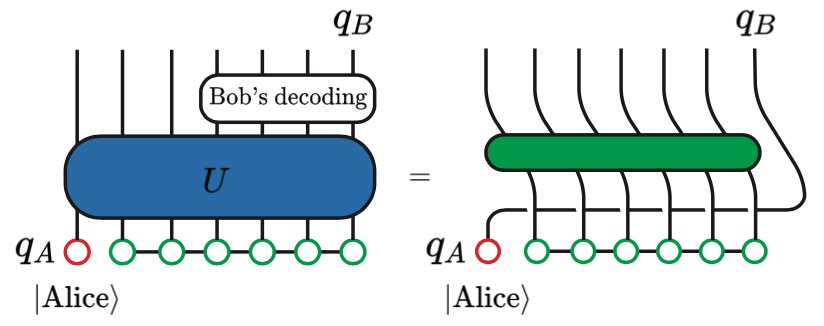
\includegraphics[align=c,width=0.6\linewidth]{pics/decode}.
\end{equation}
Denote the quantum state after the decoding $|\Psi_{\text{out}}\rangle$, the fidelity of teleporting the state $|\text{Alice}\rangle$ to the qubit $q_B$ is defined as
\begin{equation}
	F(|\text{Alice}\rangle)
	= \langle\Psi_{\text{out}}|(|\text{Alice}\rangle\langle\text{Alice}|)_{q_B} \otimes \mathbb I\left|\Psi_{\text{out}}\right\rangle .
\end{equation}
When the fidelity averaged over Alice's state $\mathbb{E}[F(|\text{Alice}\rangle]$ is 1, it indicates that the system is able to teleport any quantum state with perfect fidelity. 
The averaged fidelity can be obtained by sampling Alice's state from the action of a random unitary $u_a$ on a basis state $|0\rangle$,
\begin{equation}
	\mathbb{E}[F(|\text{Alice}\rangle] 
	= \mathbb{E}_{u_a} 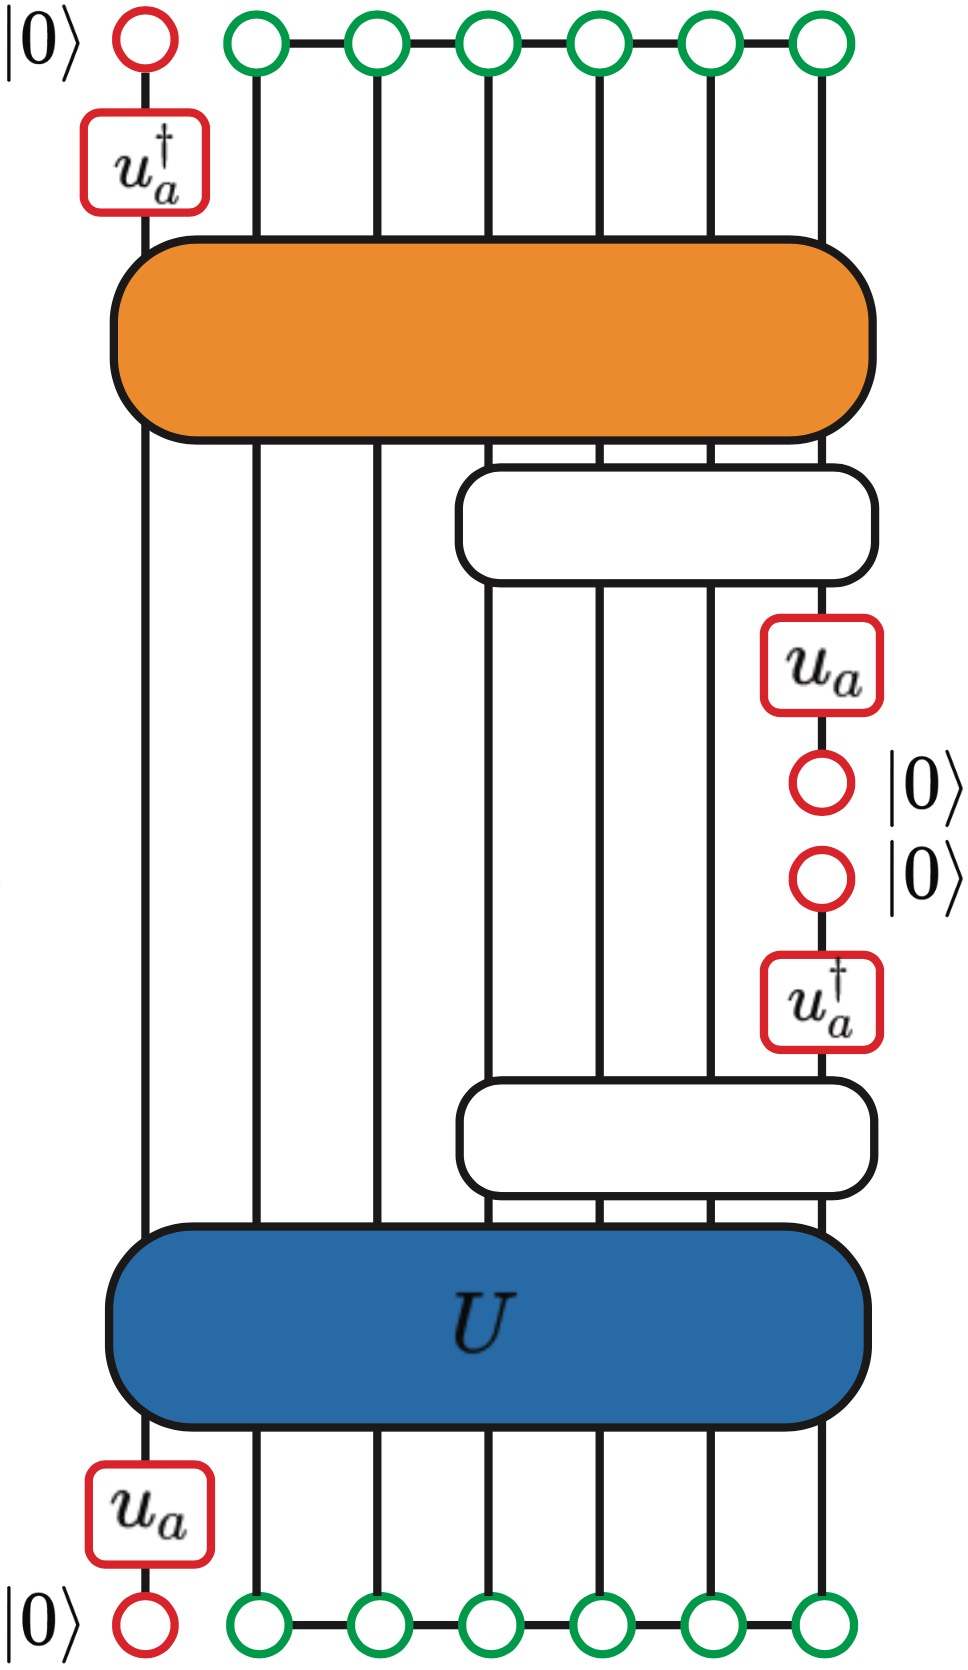
\includegraphics[align=c,width=0.2\linewidth]{pics/decode-2}
	= \frac{1}{3} + \frac{2}{3} F_\mathrm{EPR},\quad F_\mathrm{EPR} \equiv 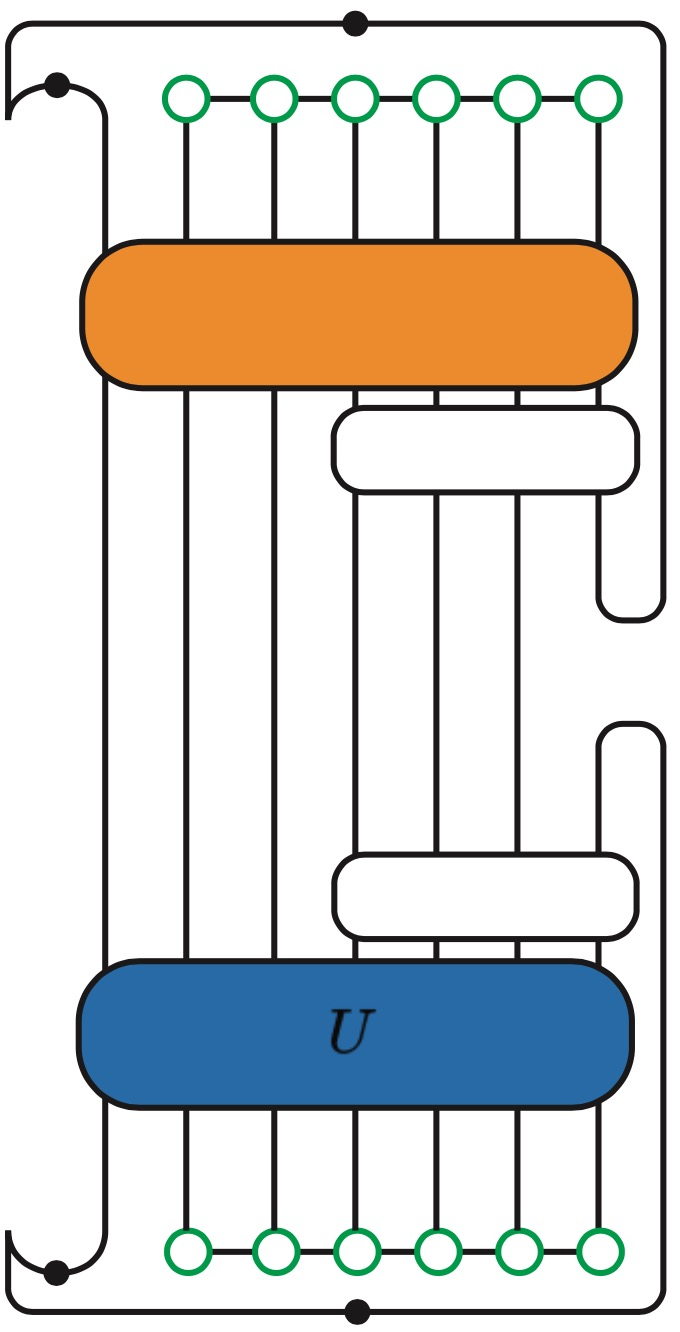
\includegraphics[align=c,width=0.18\linewidth]{pics/decode-3}.
\end{equation}
Note that the last equation comes from the averaging
\begin{equation}
\begin{aligned}
	\int_{U_2} dU \ U_{i_1 0} U_{i_1^{\prime} 0}^* U_{i_2 0} U_{i_2^{\prime} 0}^* 
	= \frac{1}{6} (\delta_{i_1 i'_1}\delta_{i_2 i'_2} + \delta_{i_1 i'_2}\delta_{i_2 i'_1}).
\end{aligned}
\end{equation}
Also, $F_\mathrm{EPR}$ can be regarded as the fidelity $F(|\text{EPR}\rangle)$ for a state initially entangled with a reference $R$ before undergoing unitary evolution.
A perfect many-body teleportation requires $F_\text{EPR}=1$.
So, before decoding, we expect the information shared between $R$ and the subsystem on which the decoder acts maximizes.

For simplicity, we first consider the case where $A_2 = q_n$ is a single qubit.
Now let us look into the mutual information $I\left(R: \operatorname{MEM} \cup q_n\right)$ more closely: $I\left(R:\mathrm{MEM} \cup q_n\right) = 2-N+S_{\mathrm{MEM} \cup q_n}$.
That is, the mutual information only depends on the entanglement entropy of $\mathrm{MEM} \cup q_n$, satisfying $N-2 \leq S\left(\operatorname{MEM} \cup q_n\right) \leq N$.
Since the Von Neumann entropy upper bounds the Renyi entropy, we have,
\begin{equation}
	I\left(R:\operatorname{MEM} \cup q_n\right) \geq 2-N+S^{(2)}_{\operatorname{MEM} \cup q_n}.
\end{equation}
Since in the case we consider here, the qubits $q_{2 \sim N}$ are in a fully mixed state, we can choose the simplest purification where the memory contains ($N-1$) auxiliary qubits that form ($N-1$) EPR pairs with the ($N-1$) spins in the system.
The time-evolved purified state is
\begin{equation}
	|\Psi\rangle = 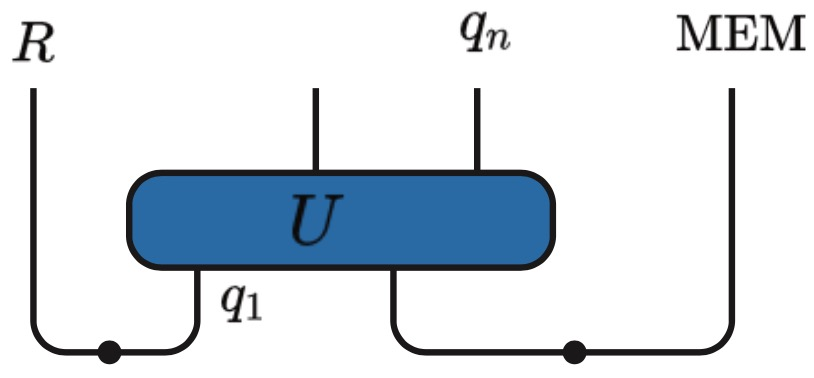
\includegraphics[align=c,width=0.28\linewidth]{pics/qn-1.jpg}, \quad
	\rho(\mathrm{MEM}\cup q_n) = \frac{1}{2}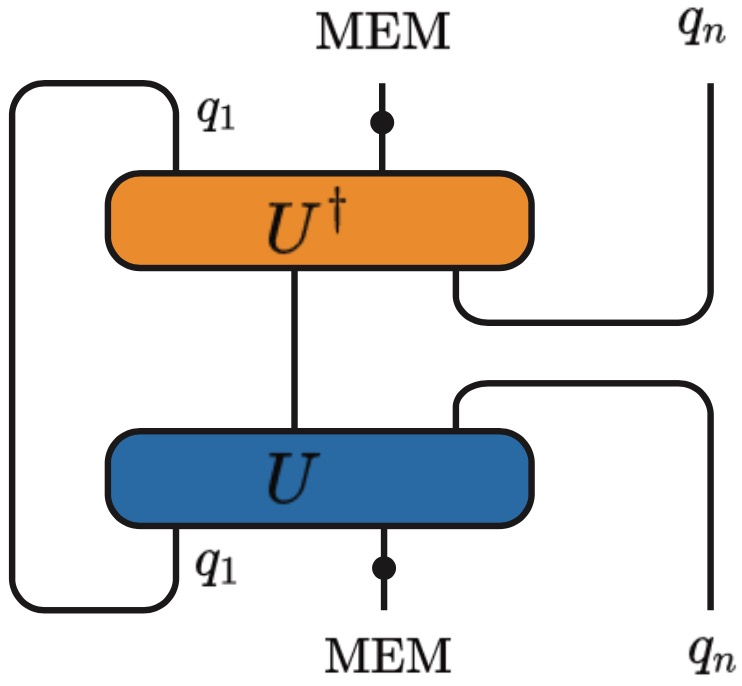
\includegraphics[align=c,width=0.22\linewidth]{pics/qn-2.jpg}.
\end{equation}
From the density matrix, we can obtain the purity $\tr\rho^2\left(\operatorname{MEM} \cup q_n\right)$ as
\begin{equation}\label{eq:purity-network}
	\tr\rho^2\left(\operatorname{MEM} \cup q_n\right) 
	= \frac{1}{4^N}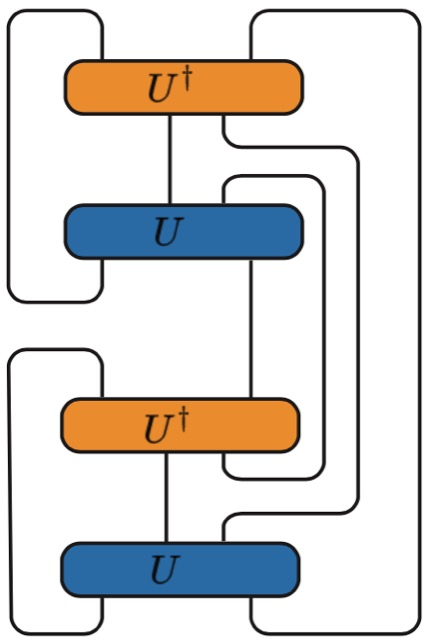
\includegraphics[align=c,width=0.18\linewidth]{pics/qn-3.jpg}
	= \frac{1}{4^{N+1}}\sum_{W,V}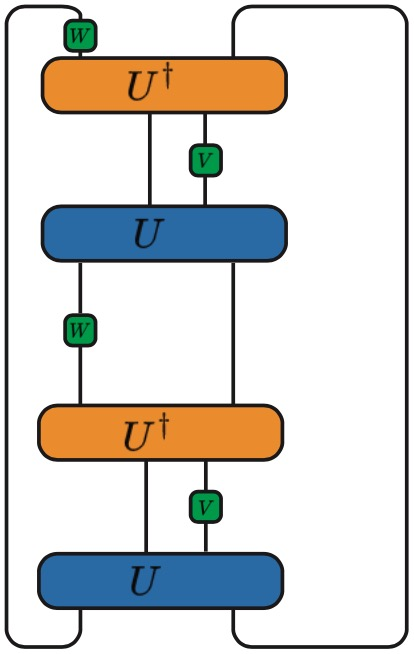
\includegraphics[align=c,width=0.18\linewidth]{pics/qn-4.jpg},
\end{equation}
where $W$ and $V$ are summed over local Pauli matrices on $q_1$ and $q_n$.
In the last equation, we used the completeness relation of Pauli operators.
When either $V_1$ or $W_n$ equals the identity, the trace contributes 1 to the sum. 
Separating these terms from the others, we get,
\begin{equation}
	\tr \rho^2\left(\operatorname{MEM} \cup q_n\right)
	= \frac{1}{2^{N+2}}\left[7+\sum_{W_1 ,V_n \neq I} \frac{1}{2^N} \tr\left(W_1(-t) V_n W_1(-t) V_n\right)\right]
\end{equation}
The purity becomes a sum of local correlators between Pauli operators. 
The Renyi entropy is just $-\log_2 \tr\left(\rho^2\right)$. 
The mutual information is then upper-bounded by the correlator
\begin{equation}
	I\left(R: \operatorname{MEM} \cup q_n\right) 
	\ge 4-\log _2\left[7+\sum_{W_1, V_n \neq I} \frac{1}{2^N} \tr\left(W_1(-t) V_n W_1(-t) V_n\right)\right].
\end{equation}
We emphasize that this inequality applies to any unitary $U$. 
Each term in the summation has the maximum value of 1, in which case the right-hand side takes the minimal value of 0. 
This happens when the Heisenberg operator $V_1(-t)$ commutes with the operator $W_n$ for all $V$ and $W$. 
When $V_1(-t)$ and $W_n$ start to overlap, the correlator decreases from 1. 
As a result, $I\left(R:\operatorname{MEM} \cup q_n\right)$ is nonzero, indicating that the information has reached $q_n$. 
At the late time, all the terms decay to 0, and the right-hand side becomes $4-\log _2 7$.



Now we discuss the decoding protocol for the Hayden-Preskill setup.
The probabilistic decoding protocol goes as follows:
\begin{enumerate}
	\item Bob takes another two qubits, $q_1^{\prime}$ and $R^{\prime}$, and prepares them in an EPR state.
	\item Bob applies the unitary operator $U^*$ to $\mathrm{MEM} \cup q_1^{\prime}$.
	\item Bob performs Bell's measurement on each qubit in $E$ and its partner in MEM, with which it forms an EPR initially.
	\item The entire protocol is repeated including preparing the state until the outcome of all the Bell measurements are the EPR states $\frac{1}{\sqrt 2}(|00\rangle+|11\rangle)$.
\end{enumerate}
After these steps, the reference $R$ and $R^{\prime}$, one of Bob's new qubits, would have high fidelity to form an EPR. 
This protocol is probabilistic because in step 3 Bob needs to post-select the EPR pairs from the Bell measurements. 
To understand this decoder, let us calculate the probability of successful postselection and the fidelity $F_{\mathrm{EPR}}\left(R, R^{\prime}\right)$ given successful postselection. 
The probability of successful postselection is
\begin{equation}
	\Delta 
	= 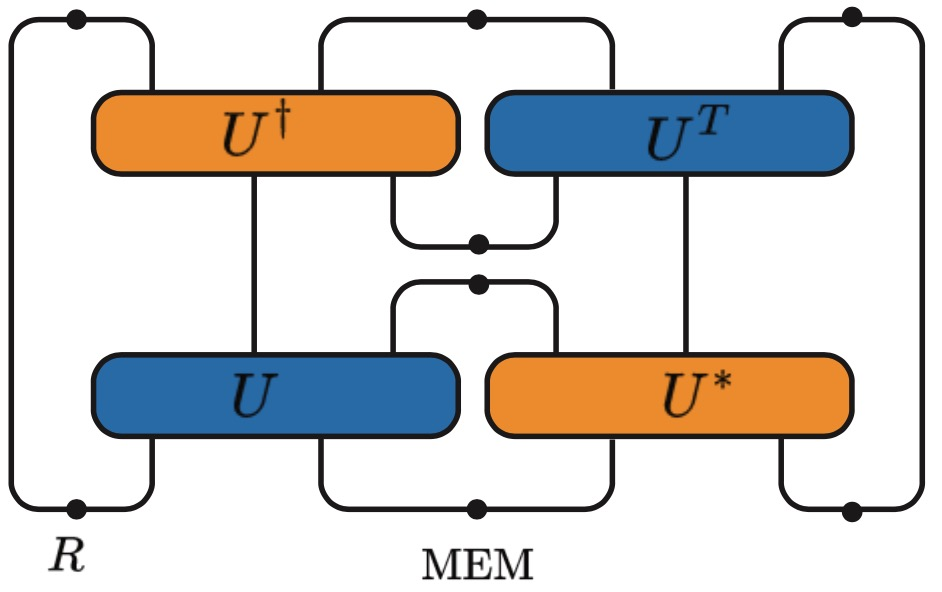
\includegraphics[align=c,width=0.25\linewidth]{pics/decode-4}
	= \frac{1}{2^{N+1+E}}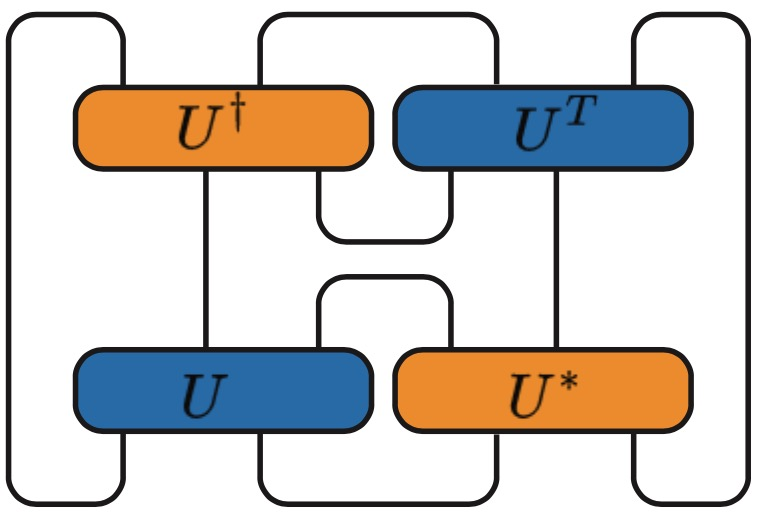
\includegraphics[align=c,width=0.22\linewidth]{pics/decode-5}.
\end{equation}
Notice that the diagram is the same as that in Eq.~(\ref{eq:purity-network}) for calculating $\rho^2(\mathrm{MEM}\cup A_2)$.
Therefore,
\begin{equation}
	\Delta = 2^{N-1-E} \operatorname{tr}^2\left(\rho_{\text{MEM}\cup A_2}\right)=2^{-I^{(2)}(R:\text{MEM}\cup E)}.
\end{equation}
The probability of the postselection is directly related to the Renyi mutual information between $R$ and Bob's qubit before the decoding. 
Given the successful postselection, the fidelity that $R$ and $R'$ form an EPR is
\begin{equation}\label{eq:EPR-fidelity}
	F_{\mathrm{EPR}} = 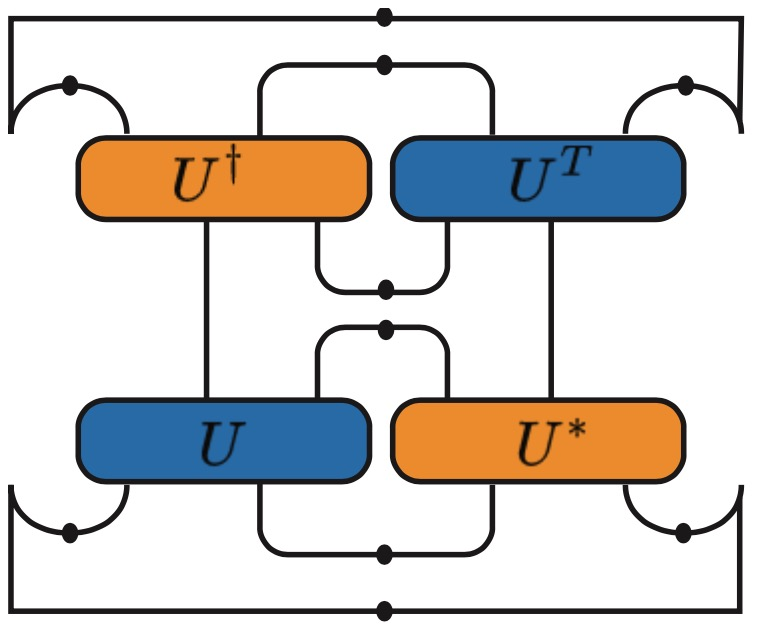
\includegraphics[align=c,width=0.2\linewidth]{pics/decode-6}/\Delta
	= 2^{I^{(2)}(R: \mathrm{MEM}\cup A_2)-2}
	= \frac{1}{1+3\times 4^{-E}}.
\end{equation}
That is, $F_{\text{EPR}}$ approach 1 exponentially fast as $E$ increases, indicating perfect teleportation fidelity given successful postselection for fully scrambling unitary time evolution. 
In general, since $\operatorname{tr}^2 \rho^2(\mathrm{MEM} \cup E)$ can be written as the sum of OTOCs as shown in Eq.~(\ref{eq:purity-network}), the fidelity $F_{\mathrm{EPR}}$ is also directly related to OTOCs as
\begin{equation}
	F_{\mathrm{EPR}} = \left[\frac{1}{4^E} \frac{1}{2^N} \sum_{W_1, V_{A_2}} \tr\left(W_1(-t) V_{A_2} W_1(-t) V_{A_2}\right)\right]^{-1},
\end{equation}
where $V_1$ and $W_{A_2}$ are summed over all local operators, including the identity, in the first qubit and $E$, respectively. 
In the fully scrambled regime, the OTOC is 1 if either $V_1$ or $W_E$ is the identity and 0 otherwise, and we get Eq.~(\ref{eq:EPR-fidelity}) back. 
We see that OTOC provides a tool to detect information propagation and is directly related to the fidelity of information recovery.




	




\section{Random Quantum Circuit}

The Haar-measure integral naturally appears in the calculation of many entanglement-related properties.
For example, when we apply a random unitary operator $U$ on (part of) the state $|\psi\rangle$, the resulting state is $|\psi'\rangle = U|\psi\rangle$.
The average of the exponential of $n$-th order renyi entropy on part $B$,
\begin{equation}\label{eq:exp-k-th-renyi}
	Z_n \equiv \left\langle q^{-(n-1)S^{(n)}_B} \right\rangle_\mathrm{Haar} 
	= \left\langle \tr \rho_B^n \right\rangle_\mathrm{Haar} 
	= \left\langle \tr_B \left(\tr_A U|\psi\rangle\langle\psi|U^\dagger\right)^n \right\rangle_\mathrm{Haar},
\end{equation}
formally takes the form of a partition function.
We can map Eq.~(\ref{eq:exp-k-th-renyi}) to an enlarged system initially at $|\Psi\rangle \equiv |\psi\rangle^{\otimes n}|\psi^*\rangle^{\otimes n}$, and the action of the unitary operator takes the form $\mathcal U = U^{\otimes n} U^{*\otimes n}$.
We regard the $2n$-fold replica indices as a new internal degree of freedom, and then the system is again a quantum chain.
The tricky part is the traces.
For a single site $i$ in part $A$, the trace is within each replica, therefore it is straightforward to check that the trace part can be equivalently expressed as the inner product with the bra:
\begin{equation}
	\langle \mathbb I |_i = \delta_{i_i \bar i_1}\cdots \delta_{i_n\bar i_n} 
	\equiv 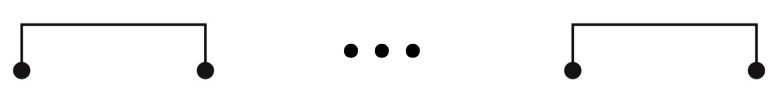
\includegraphics[align=c,width=0.25\linewidth]{pics/bra-ket-1},
\end{equation}
where we have introduced a graphic notation to represent the states.
For a site $i$ in part $B$, the 
\begin{equation}
	\langle \mathbb (12\cdots n) |_i = \delta_{i_1 \bar i_2} \delta_{i_2 \bar i_3} \cdots \delta_{i_{n-1}\bar i_n}\delta_{i_n,\bar i_1} 
	\equiv 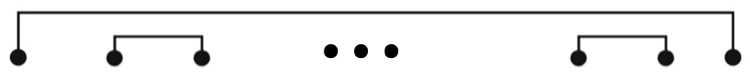
\includegraphics[align=c,width=0.25\linewidth]{pics/bra-ket-2}.
\end{equation}
The graphic notation makes the evaluation of the inner product intuitive.
For example, we have
\begin{equation}
	\langle \mathbb I|(123)\rangle 
	= 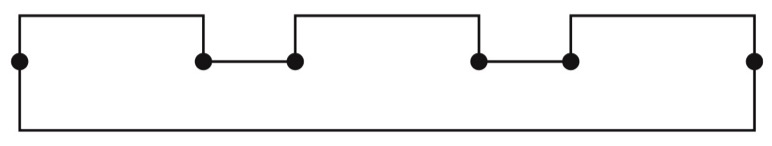
\includegraphics[align=c,width=0.2\linewidth]{pics/bra-ket-3} = q.
\end{equation}
That is, the inner product only depends on the number of cycles in permutation element $\sigma^{-1}\tau$, i.e., $\langle\sigma|\tau\rangle = q^{\#(\sigma^{-1}\tau)}$.

Assuming the unitary operator acts on sites both in $A$ and $B$, with local Hilbert space dimension $q_A$ and $q_B$ respectively.
Taking the Haar-measure average, the random unitary operator is mapped to a tensor node:
\begin{equation}\label{eq:random-unitary-gate}
	\left\langle U^{\otimes n} U^{*\otimes n} \right\rangle_\mathrm{Haar} 
	= \sum_{\sigma, \tau \in S_n} \mathrm{Wg}_{d}\left(\tau \sigma^{-1}\right)|\tau_A \tau_B\rangle\langle\sigma_A \sigma_B| 
	\equiv \sum_{\sigma, \tau \in S_n} \mathrm{Wg}_{d}\left(\tau \sigma^{-1}\right) 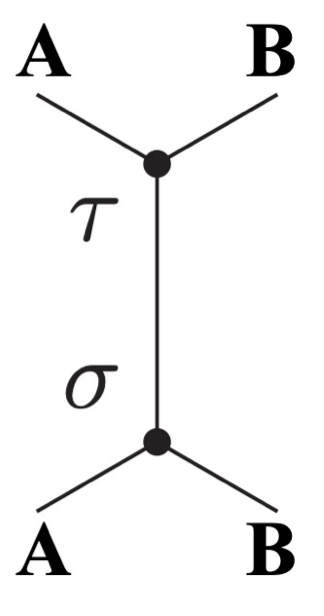
\includegraphics[align=c,width=0.05\linewidth]{pics/replica-block.jpg},
\end{equation}
where $d = q_A q_B$.

Now consider the unitary dynamics described by the random circuits:
\begin{equation}\label{eq:random-circuit}
	|\psi(t)\rangle = U_\text{circuit}(t)|\psi_0\rangle =  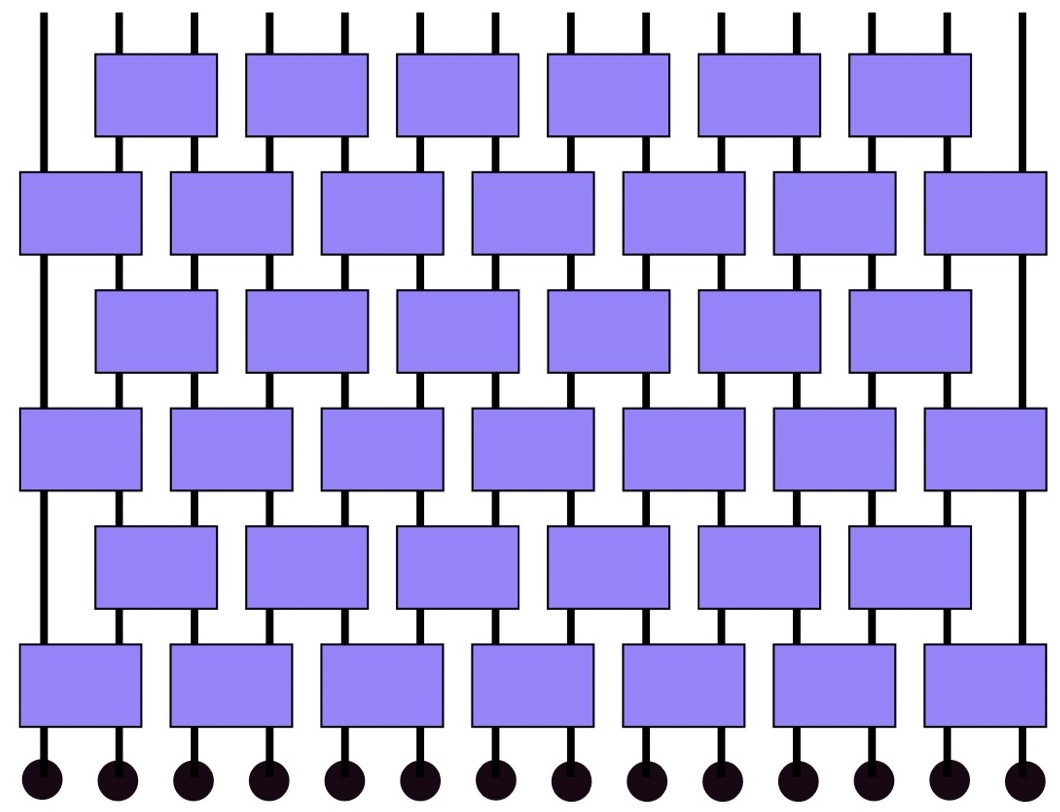
\includegraphics[align=c,width=0.3\linewidth]{pics/circuit.jpg}.
\end{equation}
As the first remark, we will show that in the $q\rightarrow \infty$ limit, a single action of a random unitary gate $U_x$ on sites $x$ and ($x+1$) will increase the zeroth-, first-, and second-order Renyi entropy maximally (we denote as $S^{(n)}_{x}$ the entropy of the first $x$ sites):
\begin{equation}
	S^{(n)}_{x}(t+1) = \min \left\{S^{(n)}_{x+1}(t+1), S^{(n)}_{x-1}(t+1)\right\}+1, \ n=0,1,2.
\end{equation}
This can be proved by showing $S^{(2)}$ approaches $S^{(0)}$ in this limit. 
We thus first define their difference as $\Delta(x, t)=S^{(0)}_x(t)-S^{(2)}_x(t) \ge 0$.
Using Eq.~(\ref{eq:alter-boundary}), which gives
\begin{equation}
	\left\langle\tr \rho_{x}(t+1)^2\right\rangle 
	= \frac{q}{q^2+1} \left\langle\tr \rho_{x+1}^2+\tr \rho_{x-1}^2\right\rangle  
	= \frac{q^2}{q^2+1}\left\langle q^{-S^{(2)}_{x+1}(t)-1}\right\rangle+\frac{q^2}{q^2+1}\left\langle q^{-S^{(2)}_{x-1}(t)-1}\right\rangle.
\end{equation}
Note that $S^{(0)}$ satisfies the maximal growth rate, which implies:
\begin{equation}
	\left\langle q^{\Delta(x, t+1)}\right\rangle < \left\langle q^{\Delta(x-1, t)}\right\rangle + \left\langle q^{\Delta(x+1, t)}\right\rangle
	\quad \Longrightarrow \quad 
	\left\langle q^{\Delta_{\max }(t+1)}\right\rangle < 2 \left\langle q^{\Delta_{\max }(t)}\right\rangle,
\end{equation}
where $\Delta_\mathrm{max}(t) \equiv \max_x \{\Delta(x,t)\}$.
We may iterate the time step successively: $\left\langle 2^{(\log_2 q)\Delta_{\text{max}}(t)}\right\rangle < 2^t$.
At fixed time $t$, as $q \rightarrow \infty$, the probability distribution for $\Delta$ concentrates around $\Delta=0$, so $S^{(2)}$ and $S^{(0)}$ agree.





\subsection{Scrambling in random circuit}

We will consider the information scrambling in the random circuit model.
The quantity we consider here is the averaged out-of-time-ordered correlator of two Pauli operators $W$ and $V$ on the sites $0$ and $x$ respectively.
This can be mapped to a tensor network by folding the evolution circuits and taking the Haar average:
\begin{equation}\label{eq:otoc-stat-model}
	F(x,t) = \frac{1}{q^N} 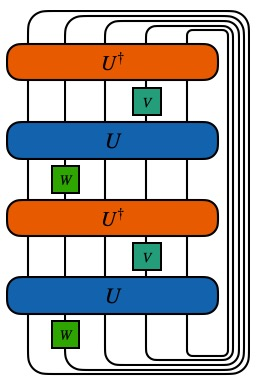
\includegraphics[align=c,width=0.15\linewidth]{pics/OTOC-1.jpg} 
	\xrightarrow{\text{ fold }} \frac{1}{q^N} 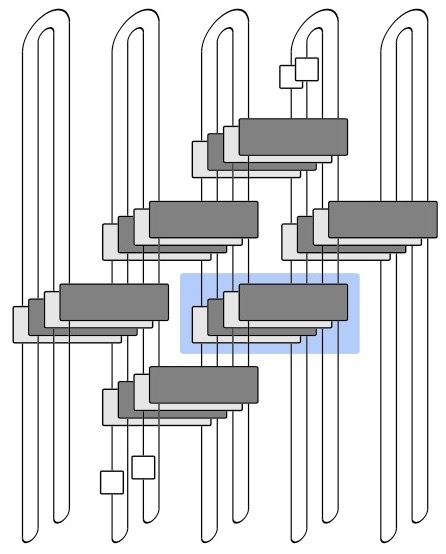
\includegraphics[align=c,width=0.17\linewidth]{pics/OTOC-3.jpg}
	\xrightarrow{\text{ average }} \frac{1}{q^N} 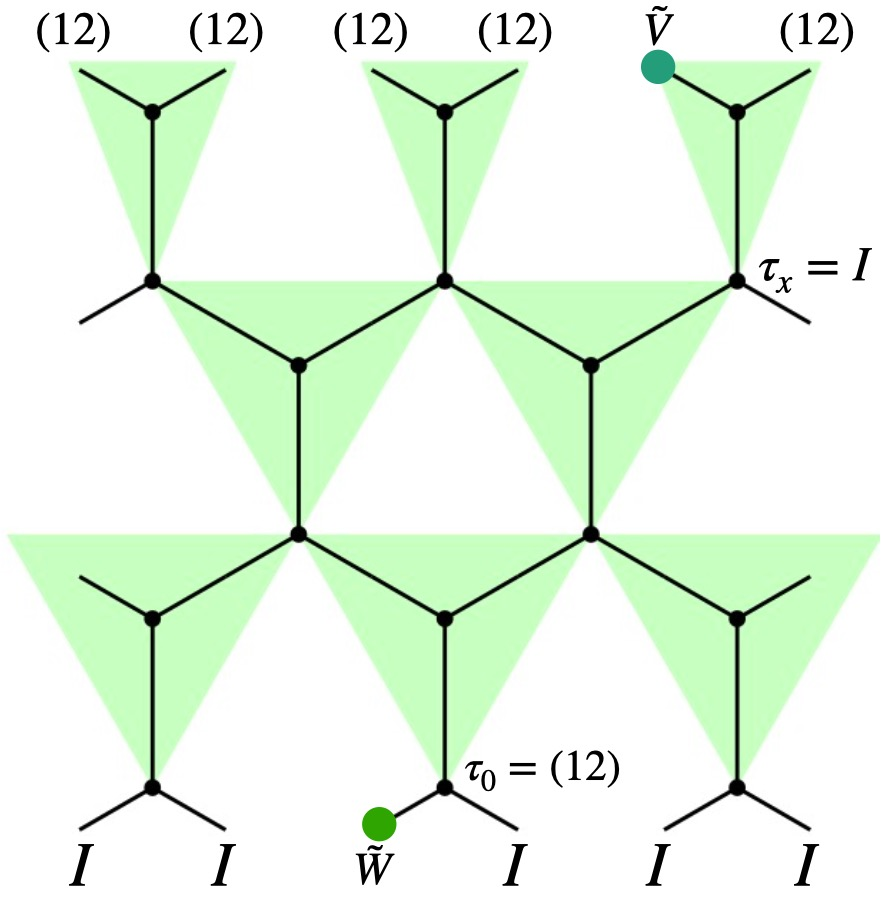
\includegraphics[align=c,width=0.23\linewidth]{pics/boundary-2},
\end{equation}
The model can be further simplified by tracing out the middle ``spin" in the green triangle.
We can then denote the weight for the resulting triangle as:
\begin{equation}
	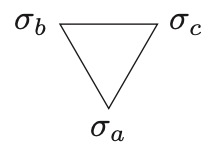
\includegraphics[align=c,width=0.1\linewidth]{pics/weight.jpg}
	= \sum_{\tau=\mathbb I, (12)} \operatorname{Wg}_d (\sigma_a \tau^{-1}) q^{\#(\sigma_b^{-1}\tau)+\#(\sigma_c^{-1}\tau)}
	=\begin{cases}
		\delta_{\sigma_a\sigma_b} & \sigma_b = \sigma_c \\
		\frac{q}{q^2+1} & \sigma_b \ne \sigma_c
	\end{cases}.
\end{equation}
This weight function makes the model behave like an Ising magnet with local sites taking values $|\mathbb I\rangle$ or $|(12)\rangle$, and subject to a special constraint: the domain wall shall not be horizontal.

For the upper boundary, if $\tau_x = (12)$, the domain wall constraint will require the whole bulk in the $|(12)\rangle$ state. 
Also, $\sigma_0 = (12)$ because $W$ is traceless.
The trick is to replace $\tilde W$ with $|\mathbb I\rangle$ and write
\begin{equation}
	F = \sum_{\tau,\tau_0=(12)} W(\tau) 
	= \sum_\tau W(\tau) - \sum_{\tau,\tau_0=\mathbb I} W(\tau)
	= 1 - \sum_{\tau,\tau_0=\mathbb I} W(\tau).
\end{equation}
In the last equation, we note the fact that $\sum_\tau W(\tau)$ is OTOC with $W$ replaced by $\mathbb I$, which is the identity.
Therefore, 
\begin{equation}
	C(x,t) = 1 - F(x,t) = \sum_{\tau,\tau_0=\mathbb I} W(\tau).
\end{equation}
When considering the statistical model corresponding to $C(x,t)$, there will be two downward domain walls starting from $x$, the total weight is nonzero only when $\tau_0$ is in the $\mathbb I$ domain.

In the bottom region, each Ising variable $\tau = (12)$ contributes a factor $q^2$, which will be renormalized out, while each $\tau=\mathbb I$ contributes a factor of $q^4$, which contribute an additional $q^2$ factor.
Since the number of Ising variables is half of the original spin, the size of the bottom domain contributes additional weight to the partition function.
Now the evaluation of the partition function is mapped to a random walk problem.
We introduce the null coordinate
\begin{equation}
	u \equiv \frac{t+x}{2}, \quad 
	v \equiv \frac{t-x}{2},
\end{equation}
and denote the endpoint in this coordinate as $(l_u, l_v)$.
For each step, either $u$ or $v$ decreases by one.
We denote the endpoint of the left/right random walk as $(l_u-u,l_v-t+u)$/$(l_u-t+v,l_v-v)$
The length of the bottom domain is $(2t-2u-2v)$.
Also, two domain walls contribute a constant factor of $\left[q/(q^2+1)\right]^{2t}$.
Therefore, the asymptotic behavior of the weight function is:\footnote{We remark here that we completely neglect the cases where two paths cross. 
Actually, the left and right domain walls correspond to two biased random walks along opposite directions. 
In the longtime limit, the crossing case is negligible.
While in the early time, the no-crossing constraint will eliminate a certain portion of the path configuration, and that is why we use the proportional expression.}
\begin{equation*}
\begin{aligned}
	C(x,t) &\propto \left(\frac{q}{q^2+1}\right)^{2t}\sum_{u=0}^{l_u} \sum_{v=0}^{l_v} q^{2t-2u-2v} 
	\begin{pmatrix} t \\ u \end{pmatrix} \begin{pmatrix} t \\ v \end{pmatrix} 
	= \left[\sum_{u=0}^{l_u}\begin{pmatrix} t \\ u \end{pmatrix} \frac{q^{2(t-u)}}{(q^2+1)^t} \right]
	\left[\sum_{v=0}^{l_v}\begin{pmatrix} t \\ v \end{pmatrix} \frac{q^{2(t-v)}}{(q^2+1)^t} \right].
\end{aligned}
\end{equation*}
Note that in the last expression, the summation corresponds to the distribution of random walk with a biased probability $p = 1/(q^2+1)$.
We know that a random walk satisfies a gaussian distribution:
\begin{equation}
	f(u) = \begin{pmatrix} t \\ u \end{pmatrix} (1-p)^{t-u} p^u
	\xrightarrow{\ x=t-2u\ } \exp\left[-\frac{1}{2}\left(\frac{x - v_B t}{\sigma(t)}\right)^2\right],
\end{equation}
where the butterfly velocity $v_B$ and the broadening factor $\sigma(t)$ are
\begin{equation}
	v_B = 1-2p = \frac{q^2-1}{q^2+1},\quad 
	\sigma(t) = \sqrt{\left[(v_B+1)^2 p + (v_B-1)^2(1-p)\right]t} = \frac{2 q \sqrt t}{q^2+1}.
\end{equation}
With proper normalization, we obtain the asymptotic expression for the OTOC:
\begin{equation}
	C(x,t) = \operatorname{erf}\left(\frac{x + v_B t}{\sigma(t)}\right) \operatorname{erf}\left(\frac{x - v_B t}{\sigma(t)}\right), \quad
	\operatorname{erf}(x) = \frac{1}{\sqrt{2\pi}} \int_{-\infty}^x e^{-\frac{x^2}{2}} dx.
\end{equation}
Thus, we have shown via an exact calculation that operator spreading in $(1+1)$D can be understood in terms of diffusion and drift. 
The front of the operator propagates at a finite velocity $v_B < 1$. 
However, the front also broadens diffusively, so its width is proportional to $\sqrt{t}$.
We conjecture that this physics also occurs in generic (nonintegrable) 1D systems undergoing deterministic Hamiltonian dynamics. 


\subsection{Entanglement entropy and replica trick}

The above mapping can be generalized to entanglement entropy.
In particular, the averaged purity entropy, defined as $\tilde S^{(2)}_x(t) \equiv -\log_q \langle \tr\rho_x^2(t)\rangle$, can be mapped to a statistical model described by a statistical model with the same bulk as Eq.~(\ref{eq:otoc-stat-model}), but with a free boundary condition on the bottom and a fixed boundary $\left\langle \mathbb I^{\otimes x},(1,2)^{\otimes (N-x)}\right|$ on the top.
In the domain-wall language, all random paths contribute equally to the partition function $Z$, i.e.,
\begin{equation}
	Z \simeq \left(\frac{2q}{q^2+1}\right)^t
	\quad\Longrightarrow\quad
	\tilde S^{(2)}_x(t) \simeq \tilde v_2 t,\quad
	\tilde v_2 =\log_q\left(\frac{q^2+1}{2q}\right).
\end{equation}
We can generalize the purity entropy to higher orders, and define $\tilde S_x^{(n)} \equiv -\frac{1}{n-1}\log_q\langle \tr\rho_x^n\rangle$.
We expect all entanglement entropies to grow linearly in time, i.e., $\tilde S^{(n)}(t) \simeq \tilde v_n t$, $S^{(n)}(t) \equiv v_n t$.
In particular, $v_1=v_E$ is called the entanglement speed.
Note that since the exponential function is convex, 
\begin{equation}
	\left\langle q^{-(n-1) S^{(n)}(t)} \right\rangle \ge q^{-(n-1)\left\langle S^{(n)}(t)\right\rangle} 
	\quad\Longrightarrow\quad
	\tilde S^{(n)}(t) \le S^{(n)}(t)
	\quad\Longrightarrow\quad
	\tilde v_n \le v_n\le v_E.
\end{equation}
Note that this expression bounds the growth rate of $S^{(n)}(t)$ but does not fix it, since the averaging of exponentials will be affected by anomalously small values of $S^{(n)}$, making it very different from $\tilde S^{(n)}$.

We can use the replica trick to access the average of Renyi entropies.
That is, we first calculate the average of $k$-th power of $Z_n \equiv \tr\rho^n_x(t)$ for an arbitrary integer number $k$.
Using the facts
\begin{equation}
	\langle Z_n^k \rangle = 1 + k \langle \ln Z_n\rangle  +\frac{k^2}{2} \langle\ln^2 Z_n\rangle + O(k^3),\quad
	\log_q(1+x) = \frac{1}{\ln q}\left(x - \frac{1}{2}x^2\right) + O(x^3),
\end{equation}
we obtain a formal series expansion for the replicated system:
\begin{equation}
\begin{aligned}
	\log_q \langle Z_n^k\rangle &=  k \frac{\langle \ln Z_n\rangle}{\ln q}  +\frac{k^2}{2} \left[\frac{\langle \ln^2 Z_n\rangle}{\ln q} - \frac{\langle\ln Z_n\rangle^2}{\ln q}\right]+ O(k^3) \\
	&= -k(n-1) \left\langle S^{(n)}(t)\right\rangle + \frac{k^2(n-1)^2 \ln q}{2}\left\langle \left[S^{(n)}(t)-\left\langle S^{(n)}(t)\right\rangle\right]^2 \right\rangle + O(k^3).
\end{aligned}
\end{equation}
That is, if we obtain the analytic form of $\left\langle Z_n^k\right\rangle$ for $k\rightarrow 0$, we not only know the averaged $n$-th order Renyi entropy, but also the variance thereof.
The full expression for $\left\langle Z_n^k\right\rangle$ is obtained by contracting the tensors (blocks) in accordance with the spatiotemporal structure of the circuit. 
Graphically, $\left\langle[\operatorname{tr}\rho_x^n]^k\right\rangle$ can be represented as a lattice magnet with a specific boundary condition, which can be graphically represented as:
\begin{equation}
	\langle Z_n^k\rangle = 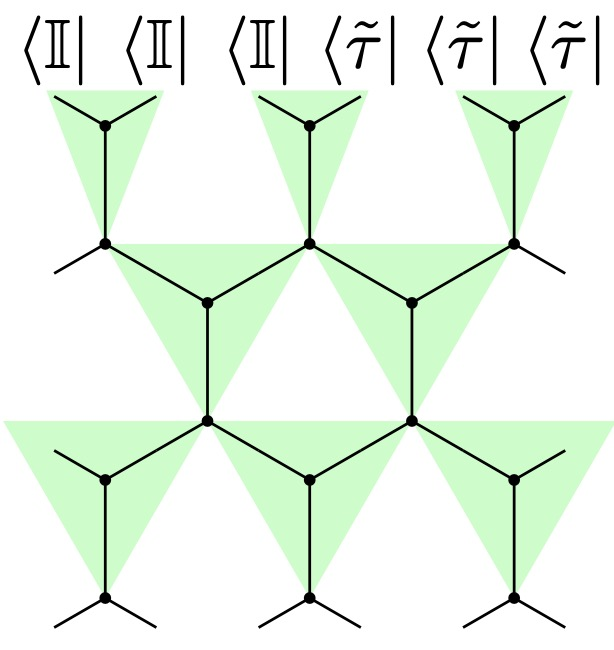
\includegraphics[align=c,width=0.18\linewidth]{pics/boundary.jpg}, \quad
	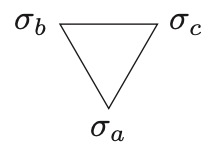
\includegraphics[align=c,width=0.12\linewidth]{pics/weight.jpg}
	= \sum_{\tau\in S_{nk}} \operatorname{Wg}_d (\sigma_a \tau^{-1}) q^{\#(\sigma_b^{-1}\tau)+\#(\sigma_c^{-1}\tau)},
\end{equation}
where on the upper boundary $|\tilde\tau\rangle = \left|(12\cdots n)^{\otimes k}\right\rangle$, and there is a free boundary condition on the bottom.








\subsection{Monitored random circuits}
Consider a random unitary circuit interspersed by local projective measurements: 
\begin{equation*}
	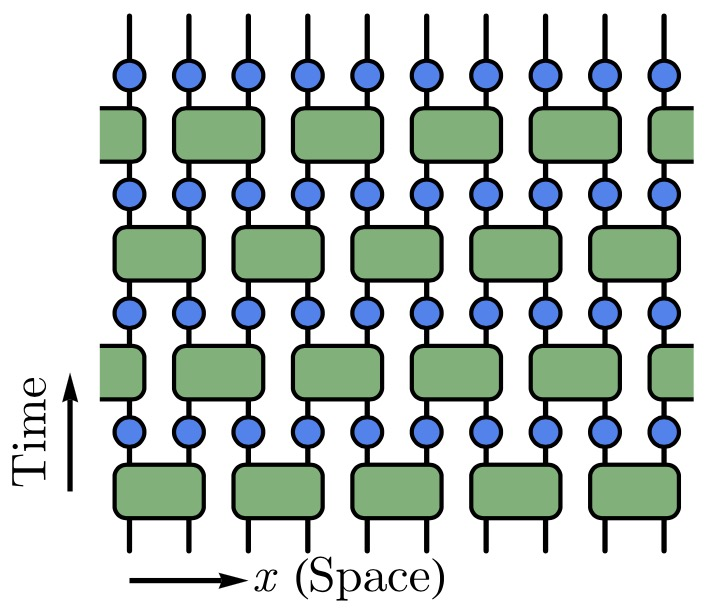
\includegraphics[align=c,width=0.25\linewidth]{pics/MIPT-1.jpg}
	\quad \Longrightarrow \quad
	Z = 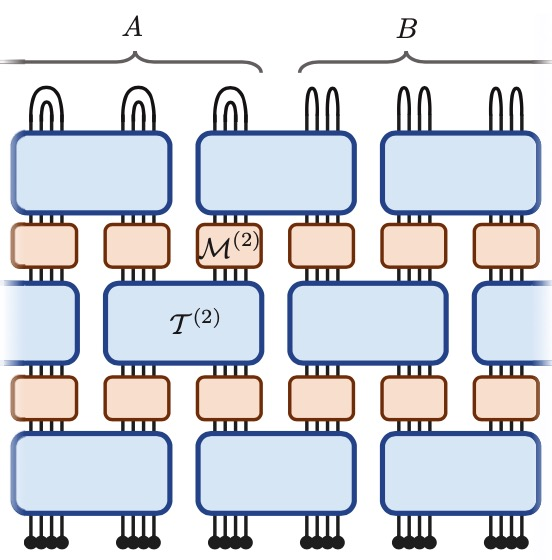
\includegraphics[align=c,width=0.25\linewidth]{pics/MIPT-2.jpg}
	\xrightarrow{\text{ average }} 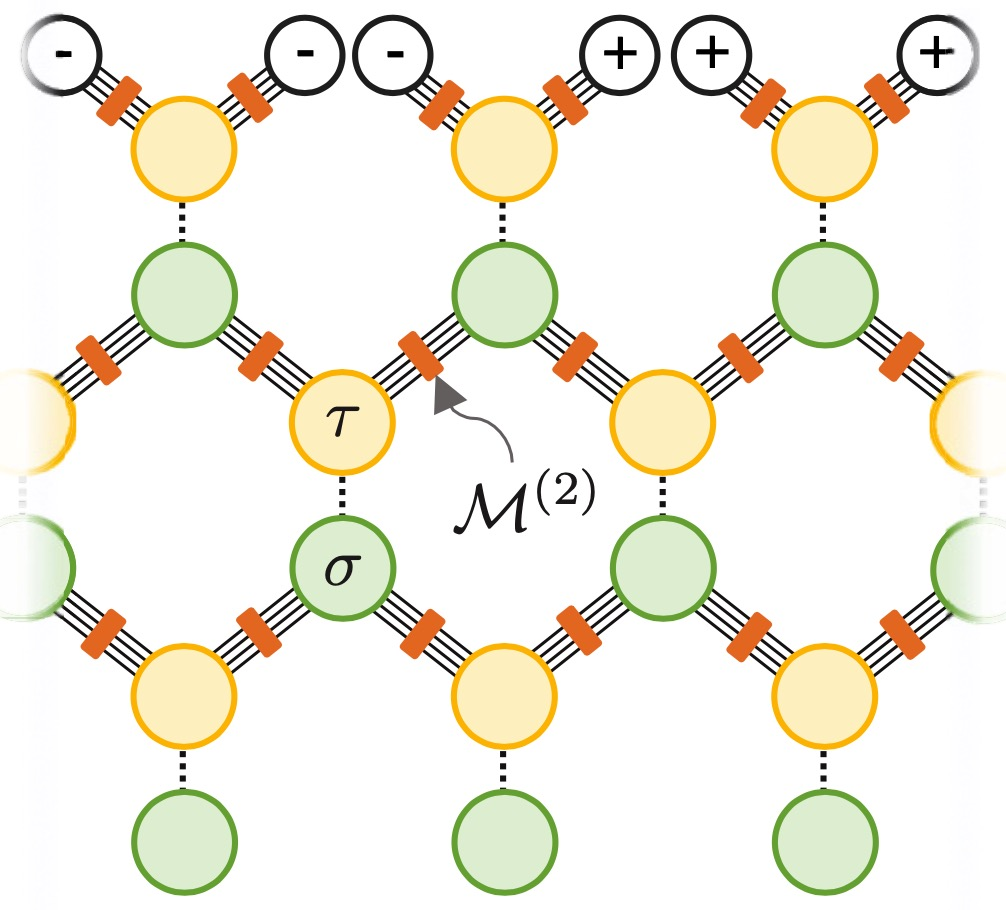
\includegraphics[align=c,width=0.25\linewidth]{pics/MIPT-3.jpg}
\end{equation*}
Each blue circle is a random measurement described by the Krause operator
\begin{equation}
	\{\mathcal M\} = \left\{\sqrt{1-p}\ \mathbb I, \sqrt p |0\rangle\langle0|,\cdots, \sqrt p|q\rangle\langle q|\right\}.
\end{equation}
We will consider the averaged purity entropy of this monitored evolution, which can also be mapped to a statistical model.
The unitary gate can be averaged similarly.
The only difference is the insertion of a quantum channel $\{\mathcal M\}$ represented by small orange bricks.
The statistical weight on the monitored bond is:
\begin{equation}
	W_p(\sigma,\tau) = \sum_{i=0}^{q} \langle \sigma|\mathcal M_i^{\otimes 4}|\tau\rangle 
	= \begin{cases}
		(1-p)q^2+pq & \sigma = \tau \\
		q & \sigma \ne \tau
	\end{cases}
	= (1-p)q^{\#(\sigma^{-1}\tau)}+pq
	\equiv W_p(\sigma^{-1}\tau).
\end{equation}
The statistical model is now a classical Ising model (with $\mathbb Z_2$ spin-flip symmetry).
We can use the Ising variables $(+) \equiv \mathbb I$, $(-) \equiv (12)$ to simplify the notation.
By integrating out the middle spin degrees of freedom, we can obtain a triangle Ising model:
\begin{equation}
	J\left(\sigma_b, \sigma_c ; \sigma_a\right)
	= \sum_{\tau=\pm} \mathrm{Wg}_d\left(\sigma_a \tau\right) W_p(\tau\sigma_b) W_p(\tau\sigma_c)
	\equiv \exp\left(-J_h\sigma_b\sigma_c-J_d \sigma_a\sigma_b-J_d \sigma_a\sigma_c\right),
\end{equation}
where the pairwise interacting strength in the horizontal/diagonal directions is $J_h$/$J_d$:
\begin{equation}
\begin{aligned}
	J(+,+;+) &= \mathrm{Wg}(+) W^2_p(+) + \mathrm{Wg}(-) W^2_p(-) = C\ e^{-J_h-2J_d}, \\
	J(-,-;+) &= \mathrm{Wg}(+) W^2_p(-) + \mathrm{Wg}(-) W^2_p(+) = C\ e^{-J_h+2J_d}, \\
	J(+,-,+) &= \left[\mathrm{Wg}(+) + \mathrm{Wg}(-)\right] W_p(+) W_p(-) = C\ e^{+J_h}.
\end{aligned}
\end{equation}
This classical model is exactly solvable.
The critical point is at
\begin{equation}
	2 e^{2J_h} = e^{-2J_d} - e^{2J_d}
	\quad \Longleftrightarrow \quad
	2J(+,-;+) = J(+,+;+) - J(-,-;+),
\end{equation}
which leads to the exact transition frequency $p_c$ for averaged purity:
\begin{equation}
	2\frac{\mathrm{Wg}(+)/\mathrm{Wg}(-)+1}{\mathrm{Wg}(+)/\mathrm{Wg}(-)-1} = \frac{W_p(+)}{W_p(-)} - \frac{W_p(-)}{W_p(+)} 
	\ \Longrightarrow \
	p_c = \frac{q^3-q^2-\sqrt{2(q^4+1)}+q+1}{(q-1) \left(q^2+1\right)}.
\end{equation}
For the qubit case ($q=2$), $p_c = (7-\sqrt{34})/5 = 0.2338\cdots$.
This transition point is smaller than the numerical result ($P_c\approx 0.26$).
We also note that in the $q\rightarrow \infty$ limit, $p_c \rightarrow 1$ apparently deviates from the percolation transition point (where $p_c=1/2$).

In the following, we will consider general $\tilde S^{(n)}$ in the $q\rightarrow \infty$ limit.
The weights $\operatorname{Wg}_{d}(\sigma)$ and $W_p(\sigma)$ in the large $q$ limit simplified to 
\begin{equation}
	\operatorname{Wg}_d(\sigma) \simeq q^{-2n} \delta_{\sigma,\mathbb I},\quad
	W_p(\sigma) \simeq (1-p)q^{n}\delta_{\sigma,\mathbb I}+pq
	\quad\Longrightarrow\quad
	J(\sigma_b,\sigma_c;\sigma_a) \simeq e^{-K(p)(\delta_{\sigma_a,\sigma_b}+\delta_{\sigma_a,\sigma_c})},
\end{equation}
where $K(p) = -\ln\left[1+\frac{1-p}{p}q^{n-1}\right] < 0$.
This is a $(nk)!$-state Potts model, whose transition point is $K_c = -\ln(1+\sqrt{n!})$.
Therefore
\begin{equation}
	p_c = \frac{q^{n-1}}{q^{n-1}+\sqrt{n!}} = \begin{cases}
		0.5 & n=1 \\
		1 & n >1 
	\end{cases}.
\end{equation}
We recover the percolation result for $S^{(1)}$.




\section{Classical Shadows}

For an unknown quantum state $\rho$, a \textbf{classical shadow} is obtained by
\begin{enumerate}
	\item Apply random unitary $U_i$ to $\rho$;
	\item Perform projective measurement on every site, which produces a vector $|b_i\rangle$;
	\item Repeat the procedure for multiple times, obtaining an ensemble $\{(U_i,|b_i\rangle)|i=1,2,\dots,N\}$.
\end{enumerate}
The expectation of $U_i^\dagger|b_i\rangle$ is a linear map of the density matrix:
\begin{equation}
	\mathcal M(\rho) 
	= \mathbb{E}\left[U^\dagger |b\rangle\langle b|U\right]
	= \sum_b \int_{U(d)} \langle b|U\rho U^\dagger|b\rangle \cdot U^\dagger |b\rangle\langle b|U.
\end{equation}
In the following, we will consider different choice twirling $\{U_i\}$.


\subsection{Global twirling}
If $U \in U(2^n)$, the Weingarten calculus returns:
\begin{equation}
	\int_{U} U_{i j_1} U_{i j_2} U_{i j_1^{\prime}}^* U_{i j_2^{\prime}}^* 
	= \frac{\delta_{j_1 j'_1}\delta_{j_2 j'_2} + 
		\delta_{j_1 j'_2}\delta_{j_2 j'_1}}{2^n(2^n+1)}.
\end{equation}
Therefore, the linear map is
\begin{equation}
	\mathcal{M}(\rho) 
= \sum_{i,\{j\}} \int_{U}  U_{i j_1}U^*_{i j_2} U_{i j_3}U^*_{i j_4}  \rho_{j_1j_2} |j_4\rangle\langle j_3| 
= \frac{\tr\rho\mathbb I+\rho}{2^n+1}.
\end{equation}
The inverse is $\mathcal{M}^{-1}(\rho) = (2^n+1)\rho - \tr(\rho)\mathbb{I}$.
For an observable $o$,
\begin{equation}
	\tr(\rho o) = \tr[\mathcal{M}(\rho)\mathcal{M}^{-1}(o)]
	= (2^n+1)\mathbb{E}\left[\langle b| U o U^\dagger |b\rangle\right] - \tr o.
\end{equation}
Note that we used the fact that $\mathcal M$ is self-adjoint since
\begin{equation*}
	\tr\left[\mathcal{M}(A)\cdot B\right] 
	= \frac{1}{d+1}\left[\tr A \tr B + \tr(AB)\right]
	= \tr\left[A\cdot\mathcal{M}(B)\right].
\end{equation*}
The classical shadow gives the sample $\hat o = \langle b|U \mathcal{M}^{-1}(o) U^\dagger|b\rangle$. The variance is
\begin{equation}
	\operatorname{Var}[\hat o] = \sum_b \int_U \langle b|U \rho U^\dagger|b\rangle 
	\langle b|U \mathcal{M}^{-1}(o) U^\dagger|b\rangle^2-[\mathbb{E}(o)]^2
	\le \left\Vert o - \frac{\tr o}{2^n}\mathbb I \right\Vert_\text{shadow},
\end{equation}
where the shadow norm is defined as
\begin{equation}
	\Vert o \Vert_\text{shadow}^2 = \max_{\sigma}\sum_b \int_U \langle b|U \sigma U^\dagger|b\rangle \langle b|U \mathcal{M}^{-1}(o) U^\dagger|b\rangle^2.
\end{equation}
We will consider the bound for the shadow norm, using the Weingarten calculus result
\begin{equation}
	\int_{U(d)} U_{i j_1} U_{i j_2}U_{i j_3} U_{i j_1^{\prime}}^* U_{i j_2^{\prime}}^* U_{i j_3^{\prime}}^* 
	= \frac{
	\delta^{j_1,j_2,j_3}_{j_1',j'_2,j'_3} + \delta^{j_1,j_2,j_3}_{j_2',j'_1,j'_3} +
	\delta^{j_1,j_2,j_3}_{j_1',j'_3,j'_2} + \delta^{j_1,j_2,j_3}_{j_3',j'_2,j'_1} +
	\delta^{j_1,j_2,j_3}_{j_2',j'_3,j'_1} +	\delta^{j_1,j_2,j_3}_{j_3',j'_1,j'_2}
	}{2^n(2^n+1)(2^n+2)}.
\end{equation}
For traceless operator $o$, the result is
\begin{equation}
	\Vert o \Vert_\text{shadow}^2 = \frac{2^n+1}{2^n+2}\max_{\sigma} \left[\tr(o^2)+2 \tr(\sigma o^2) \right] < 3 \tr(o^2).
\end{equation}
In this way, if $o$ is a projector to a certain state, the shadow norm is bounded by a constant.

\subsection{Local twirling}

If $U \in U(2)^{\otimes n}$, the linear map shall be described by the tensor product
\begin{equation}
	\mathcal{M}(o_1\otimes\cdots\otimes o_N) = \bigotimes_{i=1}^N \frac{\tr o_i\mathbb{I} + o_i}{3},\quad
	\mathcal{M}^{-1}(o_1\otimes\cdots\otimes o_N) = \bigotimes_{i=1}^N (3 o_i-\tr o_i\mathbb{I}).
\end{equation}
This map has a simple form only if the operator it acts on is a tensor product. It is suitable to predict a $k$-local Pauli operator $o = P_{i_1}\otimes\cdots\otimes P_{i_k}$:
\begin{equation}
	\tr(\rho o) = \tr[\mathcal{M}(\rho)\mathcal{M}^{-1}(o)]
	= \prod_{j=1}^k \left\{3\mathbb{E}\left[\langle b| U P_{i_j} U^\dagger |b\rangle\right] - \tr P_{i_j} \right\}.
\end{equation}
Similarly, the shadow norm is
\begin{equation}
	\Vert o \Vert_\text{shadow}^2 = \max_{\sigma} \tr\left[\sigma \bigotimes_{j=1}^k \frac{3}{4}\left(\tr P_{i_j}^2 \mathbb I+2 P_{i_j}^2 \right) \right]
	= 3^k.
\end{equation}


\end{document}
